\lesson{28}{14/05/2020} Recall that a BESQ process is characterized by an infinitesimal generator
\begin{equation}
    \mathcal{A} = 2x\dv[2]{}{x} + \delta\dv{}{x}
\end{equation}
We define the BESQ process parametrized by $\delta$ and starting from the value $x$ such that it satisfies
\begin{align}
    \dd\rho(t) &= \delta\,\dd t + 2\sqrt{\rho(t)}\,\dd W(t)
    \rho(0) &= x \ge 0
\end{align}
(where $\rho$ has nothing to do with the correlation parameter). The parameter $\delta\ge 0$ is related to the dimension of the BESQ. Another way to parametrize the process is to define the \emph{index} $\nu = \tfrac{\delta}{2}-1$:
\begin{equation*}
    \text{BESQ}^{\delta}_x = \text{BESQ}^{(\nu)}_x.
\end{equation*}
\begin{remark}
    If $\delta = n \in \mathbb{N}$ and $(W_1,\dots,W_n)$ are $n$ independent Brownian motions, then
    \begin{equation*}
        \text{BESQ}^{\delta}_x = \norm{(W_1,\dots,W_n)}
    \end{equation*}
    i.e. the BESQ is the radial distance from the origin. In fact, if we set $R(t) = \norm{W(t)}$, then
    \begin{equation*}
        R^2(t) = \sum_{i=1}^n W_i^2
    \end{equation*}
    and then
    \begin{align*}
        \dd R^2 &= n\,\dd t + \sum_{i=1}^n 2W_i\,\dd W_i \\
        &=
        n\,\dd t + 2R(t)\,\dd\bar{W}(t)
    \end{align*}
    where $\bar{W}(t)$ is the scalar Brownian motion defined as
    \begin{equation*}
        \bar{W}(t) = \frac{1}{R(t)}\sum_{i=1}^n W_i\,\dd W_i
    \end{equation*}
\end{remark} %discorso 7:00
Now, let's consider the classification of the boundary:
\begin{itemize}
    \item if $\delta \ge 2$ ($V\ge0$) then $\besqxd$ never reaches the zero (Feller condition);
    \item if $0\le\delta<2$ ($-1\le V<0$) then $\besqxd$ may reach zero, so we have to specify the boundary conditions. For the CIR process
    \begin{equation*}
        \begin{cases}
            \dd r(t) = k(\theta - r(t))\dd t + \sigma\sqrt{r(t)}\,\dd W(t) \\
            r(0) = x > 0
        \end{cases}
    \end{equation*}
    it is possible to prove that
    \begin{equation*}
        r(t) = e^{-kt}\rho\left(\frac{\sigma^2}{4k}(e^{kt}-1)\right)
    \end{equation*}
    where $\rho(t)\sim \besqxd$ with $\delta = \tfrac{4k\theta}{\sigma^2}$. Moreover, the Feller condition is given by
    \begin{equation*}
        r(t) > 0\,\, \forall t \Leftrightarrow 2k\theta \ge \sigma^2.
    \end{equation*}
\end{itemize}

\subsection{The pricing problem with stochastic volatility}
Now we consider the problem of pricing a contract in this framework. The problem is that we loose the information about the distribution of the asset price, so even if the risk neutral methodology still holds true we cannot compute conditional expected values.\\
Of course, the underlying evolves according to the B\&S formula with stochastic volatility:
\begin{equation}
    \frac{\dd S}{S} = r\,\dd t + \sqrt{V(t)}\,\dd W(t)
\end{equation}
Just for convenience, we shift from prices to returns by considering that
\begin{equation*}
    S = e^x.
\end{equation*}
Notice that $S(t)$ has an unknown distribution, so when if we want to the price of the payoff as
\begin{align*}
    price_t(\pay_T) &= e^{-r(T-t)}\expect_t[\pay_T] \\
    &=
    e^{-r(T-t)}\int_{\mathbb{R}}(e^{x_T}-K)^+ f(x_T \mid x_t)\,\dd x_T
\end{align*}
we cannot do it, because the conditional density function $f(x_T\mid x_t)$ is unknown. Since we know that there is a one to one correspondence between the density function and its Fourier transform, we can compute the density as the anti-transform of its Fourier transform:
\begin{equation*}
    \hat{f}(z) = \int_{\mathbb{R}}e^{itx}f(x\mid x_t)\,\dd x
\end{equation*}
In general $z$ is real, but we can extend $z$ to a complex domain $\mathbb{C}$ and get the so called generalized Fourier transform, also known as the Laplace transform. From the FT we can recover the density as
\begin{equation*}
    f(x_T\mid x_t) = \frac{1}{2\pi}\int_{\mathbb{R}}e^{-izx}\hat{f}(z)\,\dd t
\end{equation*}
We have that
\begin{equation*}
    \hat{f}(z) = \expect_t[e^{izx_T}]
\end{equation*}
so we can write the price of the payoff as
\begin{align*}
    price_t(\pay_T) &= e^{-r(T-t)}\int_{\mathbb{R}}(e^{x_T}-K)^+ \left(\frac{1}{2\pi}\int_{\mathbb{R}}e^{-izx_T}\hat{f}\,\dd z\right)\,\dd x_T \\
    &=
    \frac{e^{-r(T-t)}}{2\pi}\int_{\mathbb{R}}\hat{f}(z)\,\dd z \int_{\mathbb{R}}(e^{x_T}-K)^+e^{-izx}\,\dd x \\
    &=
    \frac{e^{-r(T-t)}}{2\pi}\int_{\mathbb{R}}\hat{f}(z)\hat{\pay}(-z)\,\dd z
\end{align*}
where $\hat{\pay}$ is the FT of the payoff. This integral is computed numerically. Notice that $\hat{f}(z) = \expect_t[e^{izx_T}]$ is product independent and model dependent, so once we found the characteristic function of the log-asset price in the Heston model we can use it to price whatever option (we just have to change the payoff). On the contrary, the FT of the payoff is product dependent and model independent.\\
So, the problem of pricing within the stochastic volatility framework consists in computing the integral of the product of two quantities that can be separately computed: the characteristic function of the model (which is computed only one time) and the Fourier transform of the payoff. To speed up the computation of the FT, in 1999 Carr and Madan introduced the Fast Fourier Transform in finance. \\ %discorso %fine parte 1
Let's consider some examples of payoff FT.

\subsubsection{Covered call option}
The payoff of a covered call is
\begin{equation}
    h(x_T) = \min\{e^{x_T},K\}
\end{equation}
\begin{figure}
    \centering
    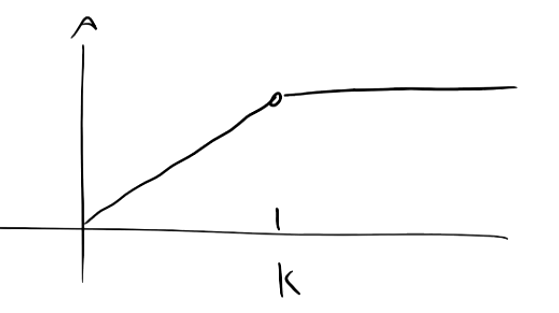
\includegraphics[scale=0.22]{fig/tmp/fig42}
    \caption{Covered call payoff.}
\end{figure}
so its FT is
\begin{align}
    \notag\hat{h}(z) &= \int_{\mathbb{R}} e^{ixz}\min\{e^x,K\}\,\dd x \\
    &=
    \notag\int_{-\infty}^{\ln K} e^{izx} e^x \,\dd x + \int_{\ln K}^{+\infty} e^{izx}K\,\dd x \\
    &=
    \eval{\frac{1}{iz+1}e^{(iz+1)x}}_{-\infty}^{\ln K} + \eval{\frac{1}{zi}e^{izx}}_{\ln K}^{+\infty}
\end{align}
In order to get convergence in the first integral, it must be
\begin{equation*}
    \Re{iz+1} > 0
\end{equation*}
so, if $z = \Re{z} + i\Im{z}$ then
\begin{equation*}
    \Re{i(\Re{z} + i\Im{z})+1} > 0 \quad\Rightarrow\quad \Im{z} < 1.
\end{equation*}
In order to get convergence in the second integral, it must be
\begin{equation*}
    \Re{iz} < 0 \quad\Rightarrow\quad \Im{z} > 0.
\end{equation*}
So, if
\begin{equation}\label{imdom}
    0 < \Im{z} < 1
\end{equation}
then we end up with
\begin{align}
    \hat{h}(z) = \frac{K^{iz+1}}{z^2-iz}.
\end{align}
\begin{figure}[h]
    \centering
    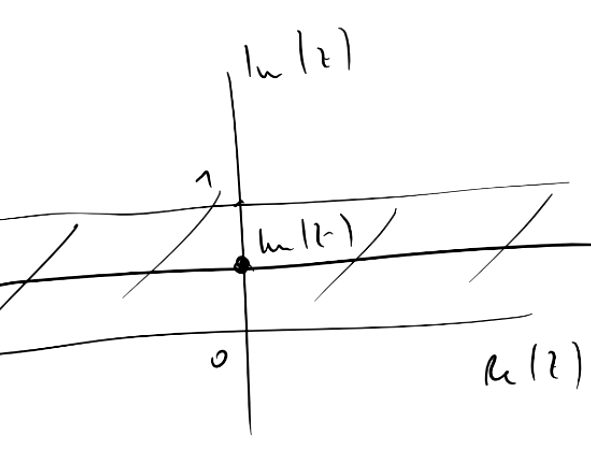
\includegraphics[scale=0.22]{fig/tmp/fig43}
    \caption{Strip of integrability.}
\end{figure}
Then the integrability domain of convergence for the (generalized) FT of the covered call will be
\begin{equation}
    \{z\in\mathbb{C}:-1<\Im{z}<0\}
\end{equation}
(the domain if the inverse of \eqref{imdom} because the argument of the payoff is $-z$).

\subsubsection{Call option}
The payoff of the call option is
\begin{equation}
    g(x_T) = (e^{x_T}-K)^+
\end{equation}
and its FT is
\begin{align}
    \notag\hat{g}(z) &= \int_{\mathbb{R}} e^{izx} (e^x-K)^+\,\dd x \\
    &=
    \eval{\frac{1}{iz+1}e^{(iz+1)x}}_{\ln K}^{+\infty}
\end{align}
In order to get convergence it must be
\begin{equation}
    \Re{iz+1} < 0 \quad\Rightarrow\quad \Im{z} > 1
\end{equation}
and provided that this condition is satisfied, the FT is given by
\begin{equation}
    \hat{g}(z) = -\frac{K^{iz+1}}{z^2-iz}.
\end{equation}
If we write $z$ as $z = a + ib$ then we have
\begin{equation*}
    \mathbb{E}[e^{-izx_T}] = \mathbb{E}[e^{bx_T}] = \mathbb{E}[S^b]
\end{equation*}
where $S$ is the underlying and $b\ge 1$. We know that, in principle, once discounted, $S$ will be a martingale, i.e. integrable. Hovever, this is not guaranteed for its moments. So we need to consider a strip of integrability such that these moments do not explode (for the B\&S model all the moments converge).

\subsubsection{Put option}
The payoff of the call option is
\begin{equation}
    g(x_T) = (K-e^{x_T})^+
\end{equation}
and its FT is
\begin{align}
    \notag\hat{g}(z) &= \int_{\mathbb{R}} e^{izx} (K-e^x)^+\,\dd x \\
    &=
    \notag \int_{-\infty}^{\ln K} e^{izx}(K-e^{x})\,\dd x \\
    &=
    \eval{\frac{K}{iz}e^{izx}}^{\ln K}_{-\infty} - \eval{\frac{1}{iz+1}e^{(iz+1)x}}_{-\infty}^{\ln K}
\end{align}
In order to get convergence it must be
\begin{align*}
    \Re{iz} > 0 &\quad\Rightarrow\quad \Im{z} < 0 \\
    \Re{iz+1} > 0 &\quad\Rightarrow\quad \Im{z} < 1
\end{align*}
so
\begin{equation}
    \Im{z} < 0
\end{equation}
Provided that this condition is satisfied, the FT is given by
\begin{equation}
    \hat{g}(z) = \frac{K^{1+iz}}{iz} - \frac{K^{iz+1}}{z^2-iz} = -\frac{K^{iz+1}}{z^2-iz}.
\end{equation}

\subsection{Characteristic functions}
What can we say about the characteristic function of the model? If
\begin{equation*}
    x_T = \ln S_T
\end{equation*}
then the characteristic function is
\begin{equation*}
    \varphi(z) = \expect_{t,x}[e^{izx_T}]
\end{equation*}
We know that in principle this guy can be also the solution of the corresponding PDE by the Feynman-Kac argument, so our guess is a function depending on the time to maturity $T-t$, on $z$, on the initial value $x$ of the process and also on a state variable $v$ related to the volatility Brownian motion:
\begin{equation*}
    \varphi(z) = G(T-t,z,x,v).
\end{equation*}
